\section{Investigation of Series and Parallel Connection}\label{sec:SimResults}

\subsection{Series Connection}

The DC bus voltage ripple of each module along with total DC bus are shown in Fig. \ref{fig:series_volt_ripple}. It has been shown that interleaving only reduces the ripple on total DC bus which has no positive effect on the modules since the module voltage ripples remain the same. Moreover, the capacitor ripple currents are not affected by interleaving since they simply have to conduct the same amount of current in series connection. Therefore, interleaving on series connection does not reduce the size of DC bus capacitors, although it is claimed so in the literature \cite{Wang2015b}. 

\begin{figure}[b]
\minipage{0.49\textwidth}
  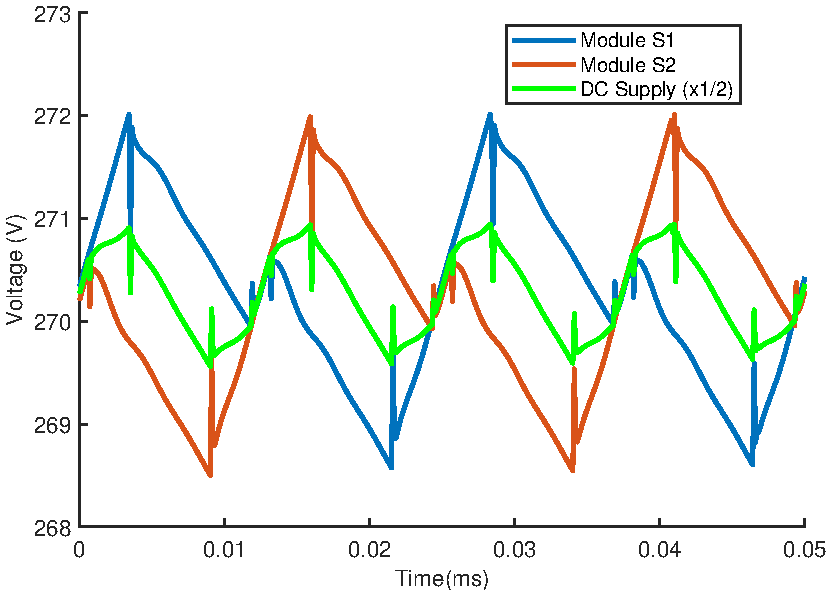
\includegraphics[width=\linewidth]{figures/series_volt_ripple.pdf}
  \caption{DC bus voltage ripple in series connected modules}\label{fig:series_volt_ripple}
\endminipage\hfill
\minipage{0.49\textwidth}
  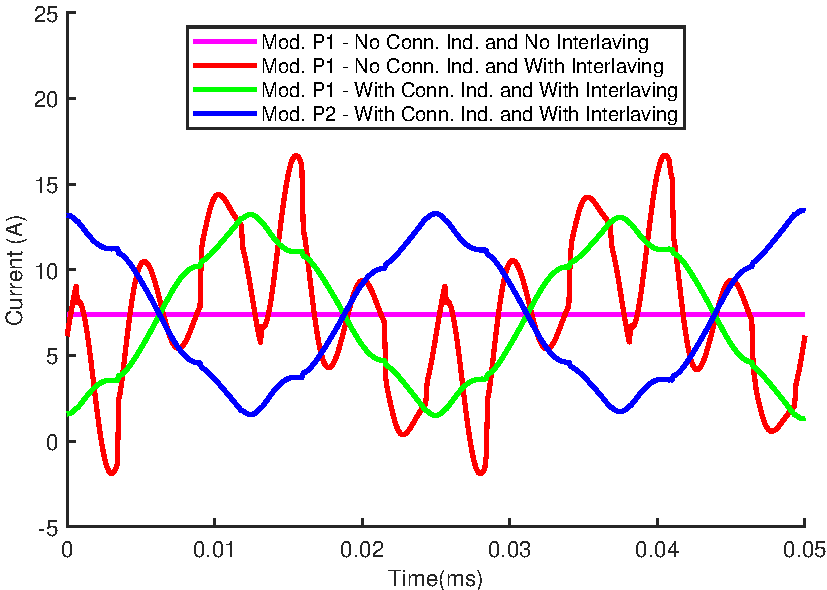
\includegraphics[width=\linewidth]{figures/parallel_current_trans.pdf}
  \caption{Current transition occuring due to interleaving in parallel connected modules}\label{fig:parallel_current_trans}
\endminipage\
\end{figure}
% Fig.7 Caption REVIEW

\subsection{Parallel Connection}

The parallel connection is usually favored to reduce the size of DC bus capacitors with interleaving. However, if the gate signals of two modules are phase shifted with proper angle, transition (circulating) currents between modules emerge, as shown in Fig. \ref{fig:parallel_current_trans}. The reduction on the capacitor current stress when interleaving is applied in parallel connected modules has been shown for different number of modules and phase shift angles in \cite{Ugur2017}. However, this analysis is only valid for ideal case where commutation and connection inductances are ignored. The RMS of capacitor currents with and without interleaving and parasitic inductances suggest that actual RMS current is larger as shown in Fig. \ref{fig:parallel_curr_rms}. On the other hand, unlike series connection, interleaving can still be used in parallel connected modules to reduce the module voltage ripple, as shown in Fig. \ref{fig:parallel_volt_ripple}.

\begin{figure}[tb]
\minipage{0.49\textwidth}
  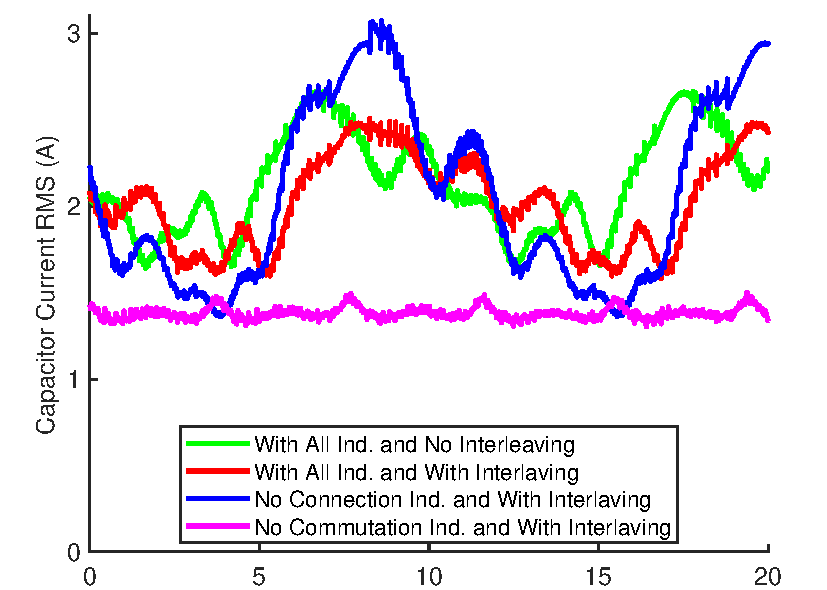
\includegraphics[width=\linewidth]{figures/parallel_curr_rms.pdf}
  \caption{Variation of DC bus capacitor current RMS in parallel connected modules}\label{fig:parallel_curr_rms}
\endminipage\hfill
\minipage{0.49\textwidth}
  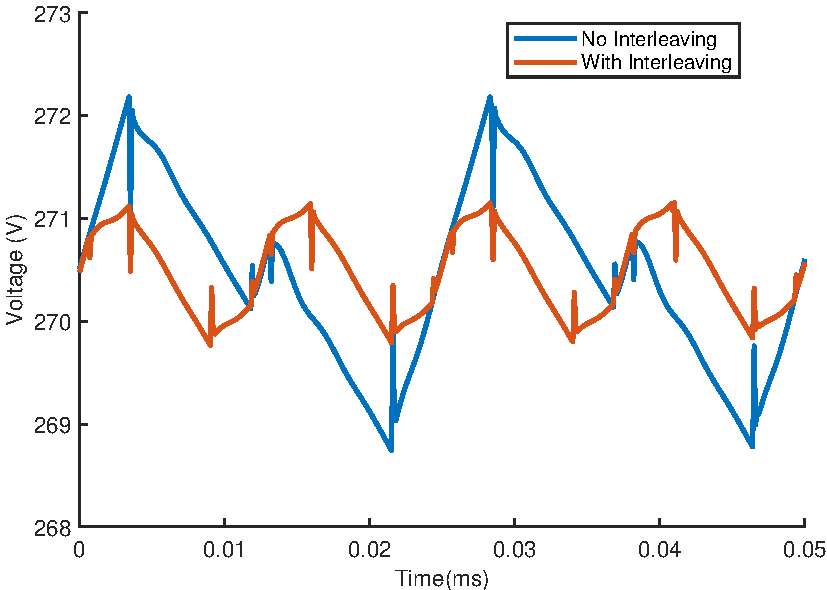
\includegraphics[width=\linewidth]{figures/parallel_volt_ripple.pdf}
  \caption{Module DC bus voltage ripple with and without interleaving in parallel connected modules }\label{fig:parallel_volt_ripple}
\endminipage
\end{figure}
